\documentclass[11pt,spanish]{article} % Tipo y tamaño de letra del documento.


\usepackage[utf8]{inputenc}
\usepackage{subfiles}
\usepackage{biblatex}
\addbibresource{references.bib}
\usepackage{multicol}
\usepackage{amsfonts}
\usepackage{blindtext}
\usepackage{mathrsfs}
\usepackage{amsmath}
\usepackage{siunitx}
\usepackage{centernot}
\usepackage[shortlabels]{enumitem}
\usepackage{subfig}
\usepackage{datetime}
\usepackage{listingsutf8}
\usepackage[spanish]{babel}
\usepackage{tikz}
\usepackage{hyperref}
\usepackage[vlined,ruled,linesnumbered]{algorithm2e}
\usepackage{listings}
\usepackage{float}
\usepackage{url}
\usepackage{csquotes}
\usepackage{fourier} %font
\usepackage[top=2cm, bottom=2cm, left=2.5cm, right=2.5cm]{geometry}
\usepackage{pgfplots}
\usepackage{fancyhdr}
\usepackage{mdframed}
\usepackage{tikzducks}
\usepackage[nameinlink]{cleveref}
\usepackage{epigraph} 

\pgfplotsset{compat=1.18}

\usetikzlibrary{shapes.arrows, shapes.geometric, arrows.meta,angles,quotes,positioning,arrows,fit,quotes,calc}
\tikzset{>=latex} 

\setlength\algomargin{1em} 
\SetFuncSty{sc} 
\SetCommentSty{em} 


\Crefname{figure}{Fig.}{Figs.}
\newcommand\crefrangeconjunction{--}
\Crefname{table}{Tabla}{Tablas}
\Crefname{subsubsection}{Subsubsec.}{Subsubsections}
\Crefname{subsection}{Subsec.}{Subsections}
\Crefname{section}{Sec.}{Sections}
\Crefname{equation}{eq.}{eqs.}
\crefname{thm}{Theorem}{theorems}
\Crefname{thm}{Theorem}{Theorems} 

\definecolor{algoco}{rgb}{0,0.4,1}

\hypersetup{
  colorlinks=true,
  linkcolor=algoco,
  citecolor=blue,
  urlcolor=blue,
}

\lstset{
extendedchars=true
inputencoding=utf8/latin1,
basicstyle=\footnotesize\sffamily\color{black},
commentstyle=\slshape \color{gray},
numbers=left,
numbersep=10pt,
numberstyle=\tiny\color{red!80!black},
keywordstyle=\color{red!80!magenta},
showspaces=false,
showstringspaces=false,
stringstyle=\color{cyan!80!black},
tabsize=2,
literate={á}{{\'a}}1 {é}{{\'e}}1 {í}{{\'i}}1 {ó}{{\'o}}1 {ú}{{\'u}}1,
frame = single, 
numbers = none,
float, floatplacement = ht, captionpos = b,
xleftmargin = 2em, xrightmargin = 2em, 
}

\newcommand{\ub}[1]{\underbrace{#1}}
\newcommand\tcm{\textcolor{magenta}}
\newcommand\tca{\textcolor{algoco}}

\setlength\epigraphwidth{.7\textwidth} 

\newcommand{\tnum}{2 y 3} % Número de la tarea
\newcommand{\sem}{2024-2} % Semestre correspondiente
\newcommand{\campus}{San Joaquín \\ Santiago} % Campus correspondiente
\newcommand{\rolusm}{202273526-0} % Rol
\newcommand{\namestudent}{Rodrigo Ramírez Díaz} % Nombre y Apellidos

\headheight=14pt
\linespread{1.3}
\author{\namestudent}
\pagestyle{fancy}
\fancyhf{}%
\fancyfoot[R]{ \namestudent \\ \rolusm}
\fancyfoot[L]{Campus \campus} 
\fancyfoot[C]{\thepage}
\rhead{2024-2}
\lhead{INF-221}
\renewcommand{\headrulewidth}{0.4pt}
\renewcommand{\footrulewidth}{0.4pt}
\newbool{programs}
\boolfalse{programs}
\chead{REPORTE TAREA \tnum~}



\title{
  \huge
  \textbf{REPORTE TAREA \tnum~ \\ ALGORITMOS Y COMPLEJIDAD} \\[1ex]
  \emph{\textquote{Explorando la Distancia entre Cadenas, una Operación a la Vez}}
  }

  
\date{
  \small
  \today\\
  \currenttime
}




\begin{document}
\maketitle
\thispagestyle{fancy} 
\vspace{-1.0\baselineskip}




\begin{abstract}
  \textit{ 
    En este informe se aborda el problema de la distancia mínima de edición extendida entre cadenas de caracteres, implementando y evaluando dos enfoques algorítmicos: \textit{Fuerza Bruta} y \textit{Programación Dinámica}. Se presentan las características principales de cada enfoque, junto con una comparación detallada de sus rendimientos en términos de tiempo de ejecución y uso de memoria, utilizando datasets diseñados específicamente para evaluar casos de transposición, semiordenados y desordenados.

La infraestructura experimental incluye la generación automatizada de datos mediante Python y la evaluación de los algoritmos implementados en C++ bajo un entorno controlado. Los resultados obtenidos destacan la ineficiencia del enfoque de \textit{Fuerza Bruta} para cadenas de longitud moderada o alta, en contraste el enfoque de \textit{Programación Dinámica}.
Este estudio subraya la importancia de seleccionar algoritmos adecuados para problemas computacionales complejos, proporcionando una base sólida para abordar problemas similares en áreas como la bioinformática y la corrección de texto.
  }
     
\end{abstract}

\setcounter{tocdepth}{1}
\tableofcontents


\newpage
\section{Introducción}
En este informe, analizaré el problema de calcular la distancia de edición entre dos cadenas de caracteres, utilizando operaciones con costos variables, como inserción, sustitución, transposición y eliminación, aplicadas una operación a la vez. Este análisis se realizará empleando dos enfoques algorítmicos distintos: Fuerza Bruta y Programación Dinámica. La elección de estos enfoques responde a la importancia de este problema en el campo del \textit{Análisis y Diseño de Algoritmos en Ciencias de la Computación}, ya que el cálculo de la distancia de edición ha permitido avances significativos en aplicaciones como la búsqueda de texto y en motores de búsqueda (por ejemplo, Google), donde es posible restringir resultados a palabras similares dentro de un margen específico de error.

Diversas investigaciones han explorado el concepto de búsqueda aproximada, en la cual se permite cierto grado de 'error' o diferencia entre dos cadenas de caracteres, una herramienta muy utilizada en áreas como la bioinformática. Un ejemplo relevante se menciona en \citetitle{MedigraphicPaper}, donde se destaca que \textit{"una de las principales herramientas que permiten la localización de características comunes en cadenas de proteínas o ADN de distintas especies es la búsqueda aproximada de cadenas."}. Esta técnica es fundamental para el análisis de secuencias biológicas, donde la distancia de edición se convierte en una métrica clave para medir similitudes y realizar comparaciones entre datos complejos.

El principal objetivo de este informe es resaltar la importancia de aplicar estos algoritmos de forma eficiente, reduciendo de manera significativa la complejidad temporal del problema, para ello se presentará una comparación en términos de velocidad entre los enfoques de Fuerza Bruta y Programación Dinámica. Además, se busca responder una de las preguntas fundamentales en el estudio de los algoritmos: \textbf{"¿Se puede hacer mejor?"}.

Con esta premisa en mente, el propósito de este informe es realizar un análisis exhaustivo del algoritmo de distancia de edición, centrándose principalmente en su análisis temporal. Para ello, se utilizarán diversas notaciones de complejidad, como la notación Big O, la más utilizada para evaluar el rendimiento de algoritmos. Este análisis permitirá explorar cómo un enfoque algorítmico distinto y más eficiente puede reducir significativamente el tiempo de ejecución, pasando de una complejidad exponencial a una lineal en ciertos casos. Además, se plantearán variaciones al problema estándar de distancia entre dos cadenas de carácteres, para evaluar si dichas variantes pueden ofrecer beneficios en aplicaciones prácticas actuales.

\newpage
\section{Diseño y Análisis de Algoritmos} 
En esta sección se diseñan dos algoritmos que buscan resolver el problema de la distancia mínima de edición extendida entre dos cadenas dadas, S1 y S2. Cada algoritmo utiliza las operaciones de inserción, sustitución, eliminación, y la variante de transposición, junto con sus respectivos costos.

El primer enfoque, \textit{"Fuerza Bruta"}, implementa una solución exhaustiva en la que se exploran todos los caminos posibles para transformar S1 en S2. En este enfoque, para hacer coincidir un solo carácter entre ambas cadenas, se generan todas las opciones posibles, lo que crea un árbol de decisiones donde cada nodo representa una operación. A medida que se avanza en cada carácter de las cadenas, el proceso se repite recursivamente para las letras restantes, evaluando todas las combinaciones de operaciones posibles. Al final, cuando se han recorrido todas las ramas del árbol, se selecciona la solución con el menor costo total.

Por ejemplo, consideremos las palabras S1 = 'amores' y S2 = 'amaras'. Al comparar los primeros caracteres de ambas cadenas, no se genera ningún conflicto; sin embargo, al llegar al tercer carácter de S1 'o' y compararlo con el tercer carácter de S2 'a', el algoritmo calcula los costos de las cuatro posibles operaciones (inserción, eliminación, sustitución y transposición) para hacer que ambos caracteres coincidan. Cada una de estas operaciones genera una llamada recursiva para el resto de la cadena, resultando en cuatro ramificaciones desde este punto en el árbol.

Este proceso continúa a medida que avanzamos en las cadenas, y al comparar el quinto carácter de S1 'e' con el quinto de S2 'a', cada una de las cuatro ramificaciones previas vuelve a generar otras cuatro, ya que cada rama evalúa nuevamente las cuatro operaciones posibles. Esto resulta en un árbol de decisiones con 16 nodos hoja hasta este punto.

Este proceso puede visualizarse más fácilmente en la siguiente \cref{fig:arbol-fuerza-bruta} del diagrama del árbol resultante, que ilustra el crecimiento exponencial de las llamadas recursivas en el enfoque de Fuerza Bruta:


 \begin{itemize}
     \item \textbf{Análisis Temporal}
     
     El análisis temporal del algoritmo de Fuerza Bruta, en el peor de los casos, considera que se deben calcular los costos para cada carácter de la cadena S1. A medida que se avanza en cada carácter, se generan cuatro ramificaciones (una para cada operación: inserción, eliminación, sustitución y transposición), lo cual expande exponencialmente el árbol de decisiones. Si consideramos que la longitud de S1 es \( n \), entonces el árbol resultante tendrá aproximadamente \( 4^n \) nodos en el peor de los casos, dado que cada operación genera cuatro posibles caminos a seguir. Por lo tanto, la complejidad temporal del algoritmo es \( O(4^n) \), lo que lo convierte en un método ineficiente para cadenas largas debido a su crecimiento exponencial en tiempo de ejecución.

    \item \textbf{Análisis Espacial}

    En cuanto al análisis espacial, la cantidad de espacio requerida difiere del crecimiento temporal. En el algoritmo de Fuerza Bruta, cada llamada recursiva crea una copia de las cadenas restantes en la pila de ejecución, pero el almacenamiento de datos solo requiere guardar los caracteres de S1 y S2 en el nivel actual de la recursión. Esto significa que, en el primer nivel (la raíz del árbol de decisiones), se necesita espacio para \( n \) caracteres. A medida que se desciende en el árbol y se realizan llamadas recursivas, el espacio utilizado por cada nivel se reduce, ya que las cadenas a comparar disminuyen en tamaño. 

    Por lo tanto, en el último nivel, correspondiente a los nodos hoja, se almacenan únicamente las operaciones finales sobre caracteres individuales. Esto implica que el espacio máximo en la pila de ejecución está limitado por la profundidad del árbol, que es \( n \), resultando en una complejidad espacial de \( O(n) \).

 \end{itemize}

  \begin{figure}[H]
    \centering
    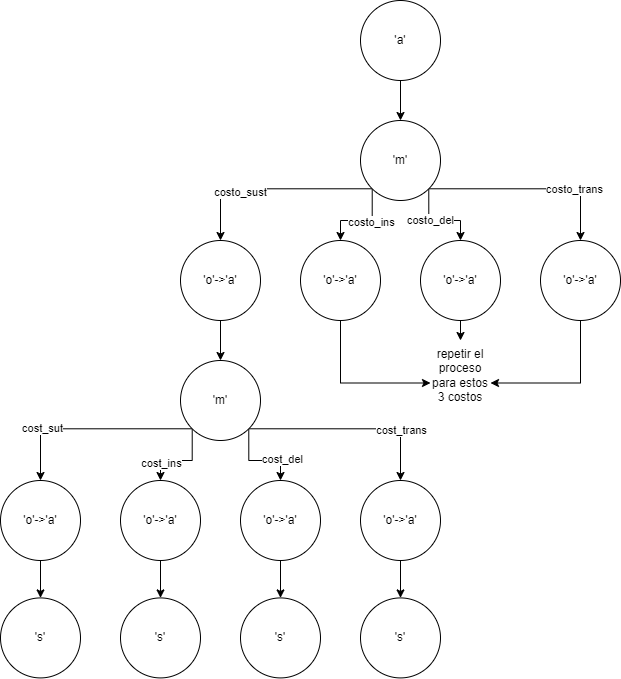
\includegraphics[width=0.9\linewidth]{images/ejemplo_fuerza_bruta.png}
    \caption{Diagrama del arbol implicito que resulta de la ejecucion del prgrama \textit{brute\_fi.py}.}
    \label{fig:arbol-fuerza-bruta}
 \end{figure}
 

\subsection{Fuerza Bruta}

\epigraph{\textit{``Indeed, brute force is a perfectly good technique in many cases; the real question is, can we use brute force in such a way that we avoid the worst-case behavior?''}}{--- \citeauthor{taocv3}, \citeyear{taocv3} \cite{taocv3}}

\begin{algorithm}[H]
    \SetKwProg{myproc}{Procedure}{}{}
    \SetKwFunction{AlgorithmName}{AlgorithmName}  % Cambia 'AlgorithmName' por el nombre del enfoque elegido
    \SetKwFunction{AuxiliaryFunction}{AuxiliaryFunction}  % Función auxiliar de ejemplo
    
    \DontPrintSemicolon
    \footnotesize

    % Definición del algoritmo principal
    \myproc{\AlgorithmName{S1, S2}}{
    \uIf{S1 está vacía}{
        \Return longitud de S2\;  % Return explícito si S1 está vacía
    }
    \uElseIf{S2 está vacía}{
        \Return longitud de S1\;  % Return explícito si S2 está vacía
    }
    \uElseIf{S1[0] = S2[0]}{
        \Return \AlgorithmName{S1[1:], S2[1:]}  % Llamada recursiva
    }
    \Else{
        % Ejemplo de llamado a una función auxiliar
        $costo \leftarrow \AuxiliaryFunction{S1, S2}$\;
        \Return costo\;  % Retornar el valor calculado
    }
    }

    % Definición de la función auxiliar
    \myproc{\AuxiliaryFunction{S1, S2}}{
    % Acciones o cálculos auxiliares
    \uIf{S1 y S2 son similares}{
        \Return algún valor o costo\;  % Retornar el valor calculado por la función auxiliar
    }
    \Else{
        % Llamar de nuevo a la función principal
        \Return \AlgorithmName{S1 modificado, S2}\;  % Llamada recursiva y retorno del resultado
    }
    }
    \caption{Este es solo un ejemplo de cómo estructurar el pseudocódigo, con retornos explícitos y llamados a funciones.}
    \label{alg:mi_algoritmo_1}
\end{algorithm}
\subsection{Programación Dinámica}
\epigraph{\textit{Dynamic programming is not about filling in tables. It's about smart recursion!}}{\citeauthor{algorithms_erickson}, \citeyear{algorithms_erickson} \cite{algorithms_erickson}}


\subsubsection{Descripción de la solución recursiva}

La solución por programación dinámica se implementa usando una estrategia de tabulación (enfoque \textit{Bottom-Up}), en la cual se utiliza una matriz para almacenar los costos de cada operación de edición (inserción, eliminación, sustitución y transposición) entre caracteres de las cadenas \texttt{S1} y \texttt{S2}. La matriz tiene dimensiones \( 4 \times N \), donde \( N \) representa la longitud de \texttt{S1} y el valor 4 corresponde a las cuatro operaciones posibles.

Para calcular la distancia mínima, se rellena la matriz por columnas. Cada columna representa el costo acumulado de transformar un carácter de \texttt{S1} en el carácter correspondiente de \texttt{S2} mediante una de las operaciones. El primer elemento de cada columna se inicializa en 0 si los caracteres de \texttt{S1} y \texttt{S2} son iguales, ya que no requiere ninguna operación; en caso contrario, se calcula su costo.

Para la siguiente fila (operación de costo mínimo para el mismo carácter), se evalúa el costo y se almacena el mínimo entre el costo calculado y el costo acumulado de la operación anterior. Este proceso asegura que cada columna contenga el costo mínimo de las cuatro operaciones para un carácter dado, y además, se suma el costo acumulado de la columna anterior para reflejar el costo de transformación secuencial. Al finalizar, el valor en la última celda de la matriz representa el costo mínimo o distancia de edición entre las dos cadenas.

\subsubsection{Relación de recurrencia}

La relación de recurrencia establece el costo mínimo para transformar un prefijo de \texttt{S1} en un prefijo de \texttt{S2}. Se define como:
\[
D(i, j) = \min \begin{cases} 
      D(i-1, j) + \text{COSTO\_DEL}(\texttt{S1}[i-1]) & \text{(eliminación)} \\
      D(i, j-1) + \text{COSTO\_INS}(\texttt{S2}[j-1]) & \text{(inserción)} \\
      D(i-1, j-1) + \text{COSTO\_SUB}(\texttt{S1}[i-1], \texttt{S2}[j-1]) & \text{(sustitución)} \\
      D(i-2, j-2) + \text{COSTO\_TRANS}(\texttt{S1}[i-2], \texttt{S1}[i-1]) & \text{(transposición)}
   \end{cases}
\]
con los casos base:
\[
D(i, 0) = i \cdot \text{COSTO\_DEL}(\texttt{S1}[i-1])
\]
\[
D(0, j) = j \cdot \text{COSTO\_INS}(\texttt{S2}[j-1])
\]
\\
\subsubsection{Identificación de subproblemas}

Cada subproblema consiste en calcular el costo mínimo de transformar un prefijo de \texttt{S1} en un prefijo de \texttt{S2}. Esto se traduce en encontrar la mínima cantidad de operaciones para cada prefijo de longitud \( i \) y \( j \) de \texttt{S1} y \texttt{S2}, respectivamente. Al resolver estos subproblemas y almacenarlos en la matriz, se evita la recalculación redundante y se optimiza el cálculo de la solución final.

\subsubsection{Estructura de datos y orden de cálculo}

La estructura de datos utilizada es una matriz bidimensional \( D[i][j] \), donde \( D[i][j] \) almacena el costo mínimo para transformar el prefijo de longitud \( i \) de \texttt{S1} en el prefijo de longitud \( j \) de \texttt{S2}. La matriz se rellena secuencialmente desde la esquina superior izquierda hasta la esquina inferior derecha, asegurando que cada valor \( D[i][j] \) dependa únicamente de valores previamente calculados.

\subsubsection{Algoritmo utilizando programación dinámica}

\begin{algorithm}[H]
    \SetKwProg{myproc}{Procedure}{}{}
    \SetKwFunction{DistanciaMinima}{DistanciaMinima}
    
    \DontPrintSemicolon
    \footnotesize

    % Definición del algoritmo principal
    \myproc{\DistanciaMinima{S1, S2}}{
        $n \leftarrow \text{longitud de } S1$\;
        $m \leftarrow \text{longitud de } S2$\;
        Crear matriz $D$ de tamaño $(n+1) \times (m+1)$\;
        
        \For{$i \leftarrow 0$ \KwTo $n$}{
            $D[i][0] \leftarrow i \times \text{COSTO\_DEL}(S1[i-1])$\;
        }
        \For{$j \leftarrow 0$ \KwTo $m$}{
            $D[0][j] \leftarrow j \times \text{COSTO\_INS}(S2[j-1])$\;
        }
        
        \For{$i \leftarrow 1$ \KwTo $n$}{
            \For{$j \leftarrow 1$ \KwTo $m$}{
                $costo\_del \leftarrow D[i-1][j] + \text{COSTO\_DEL}(S1[i-1])$\;
                $costo\_ins \leftarrow D[i][j-1] + \text{COSTO\_INS}(S2[j-1])$\;
                $costo\_sub \leftarrow D[i-1][j-1] + \text{COSTO\_SUB}(S1[i-1], S2[j-1])$\;
                
                \uIf{$i > 1 \land j > 1 \land S1[i-1] = S2[j-2] \land S1[i-2] = S2[j-1]$}{
                    $costo\_trans \leftarrow D[i-2][j-2] + \text{COSTO\_TRANS}(S1[i-2], S1[i-1])$\;
                }
                \Else{
                    $costo\_trans \leftarrow \infty$\;
                }
                
                $D[i][j] \leftarrow \min(costo\_del, costo\_ins, costo\_sub, costo\_trans)$\;
            }
        }
        \Return $D[n][m]$\;
    }
    \caption{Algoritmo de Programación Dinámica para la distancia mínima de edición entre dos cadenas.}
    \label{alg:mi_algoritmo_pd}
\end{algorithm}

\newpage
\section{Implementaciones}
\begin{mdframed}
    \textbf{La extensión máxima para esta sección es de 1 página.}
\end{mdframed}

Aquí deben explicar la estructura de sus programas haciendo referencias a los archivos y funciones de su entrega. No adjunte código en esta sección.
\begin{mdframed}
    Si se utiliza algún código, idea, o contenido extraído de otra fuente, este \textbf{debe} ser citado en el lugar exacto donde se utilice, en lugar de mencionarlo al final del informe.
\end{mdframed}

\newpage
\section{Experimentos}
\epigraph{``\textit{Non-reproducible single occurrences are of no significance to science.}''}{---\citeauthor{popper2005logic}, \citeyear{popper2005logic} \cite{popper2005logic}}

En esta sección de Experimentos, analizaremos y compararemos los tiempos de ejecución y la memoria utilizada por los algoritmos implementados, utilizando gráficos que nos ayuden a visualizar las diferencias significativas entre los enfoques de \textit{Fuerza Bruta} y \textit{Programación Dinámica}. 

\subsubsection{Configuración de los Experimentos}

La recopilación de datos se realiza desde el momento en que se llaman las funciones implementadas en los archivos correspondientes. Estas funciones reciben como parámetros dos cadenas, \( S1 \) y \( S2 \), que representan los datos de entrada. Una vez que la función finaliza su ejecución, se obtienen los siguientes datos de salida:
- La distancia mínima necesaria para transformar \( S1 \) en \( S2 \).
- El tiempo de ejecución medido en segundos y microsegundos.
- La cantidad de memoria gestionada en bytes, recopilada mediante la herramienta \textbf{Valgrind} en el campo \textit{bytes allocated}.

Un ejemplo de ejecución se puede observar en la \cref{fig:ejemplo-ejecución}:

\begin{figure}[H]
    \centering
    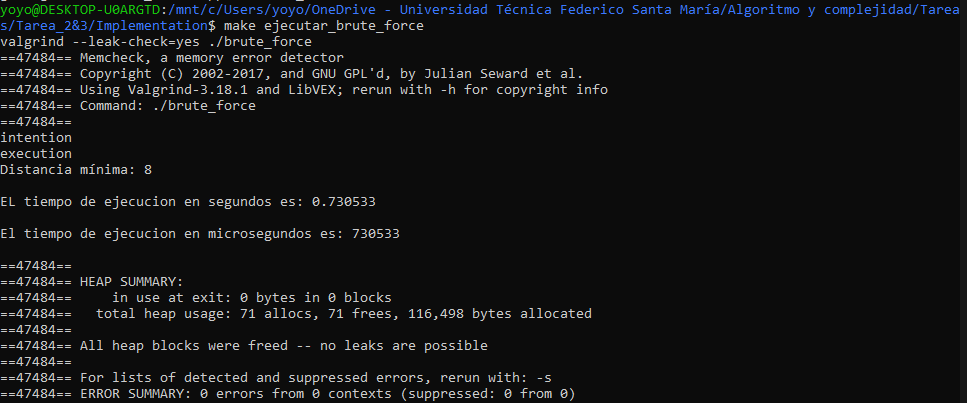
\includegraphics[width=0.75\linewidth]{Tarea_2&3//images/ejemplo_ejecucion.png}
    \caption{Ejemplo de la ejecución del programa con sus respectivas entradas y salidas.}
    \label{fig:ejemplo-ejecución}
\end{figure}

\subsubsection{Entorno de Pruebas}

Para llevar a cabo los experimentos, se utilizó el siguiente hardware y software:

\textbf{Hardware:}
  - Procesador: Intel Core i5-5200U, 2.20 GHz.
  - Memoria RAM: 12 GB.
  - Almacenamiento: Sin SSD.

\textbf{Software:}
  - Sistema Operativo: Windows 10.
  - Terminal: Ubuntu 22.04.3 LTS (en entorno WSL).
  - Compilador: \texttt{g++ 11.4.0}.
  - Librerías utilizadas:
    \texttt{<bits/stdc++.h>}, \texttt{<sys/time.h>}

Esta configuración asegura una ejecución reproducible de los experimentos, permitiendo contrastar los resultados en términos de tiempos de ejecución y uso de memoria bajo condiciones controladas.
\subsection{Dataset (casos de prueba)}
\begin{mdframed}
    \textbf{La extensión máxima para esta sección es de 2 páginas.}
\end{mdframed}
Es importante generar varias muestras con características similares para una misma entrada, por ejemplo, variando tamaño del input dentro de lo que les permita la infraestructura utilizada en ests informe, con el fin de capturar una mayor diversidad de casos y obtener un análisis más completo del rendimiento de los algoritmos.

\begin{mdframed}
    Aunque la implementación de los algoritmos debe ser realizada en C++, se recomienda aprovechar otros lenguajes como Python para automatizar la generación de casos de prueba, ya que es más amigable para crear gráficos y realizar análisis de los resultados. Python, con sus bibliotecas como \texttt{matplotlib} o \texttt{pandas}, facilita la visualización de los datos obtenidos de las ejecuciones de los distintos algoritmo bajo diferentes escenarios.
\end{mdframed}    

\begin{mdframed}    
    Debido a la naturaleza de las pruebas en un entorno computacional, los tiempos de ejecución pueden variar significativamente dependiendo de factores externos, como la carga del sistema en el momento de la ejecución. Por lo tanto, para obtener una medida más representativa, siempre es recomendable ejecutar múltiples pruebas con las mismas características de entrada y calcular el promedio de los resultados.
\end{mdframed}

\subsection{Resultados}
En esta sección se presentan los resultados de ambos enfoques algorítmicos mediante gráficos de dispersión, considerando los costos y archivos de entrada disponibles en el repositorio de GitHub referenciado en la sección de Implementación. Cabe destacar que estos archivos no han sido ni serán modificados, lo que permite verificar la reproducibilidad de los resultados.

Para replicar los experimentos, basta con ejecutar los comandos \texttt{make} mencionados anteriormente, ingresando manualmente los datos de entrada que se encuentran en los archivos \texttt{.txt}. Aunque sería posible automatizar todos los casos mediante \texttt{make}, esto haría el proceso innecesariamente complejo y menos flexible para el usuario, limitando la posibilidad de probar casos específicos de forma manual. Para detalles sobre la compilación y ejecución de los programas \texttt{.cpp}, puede utilizar el comando \textbf{\texttt{make help}} en la terminal. Es importante asegurarse de que el sistema tenga un compilador compatible con archivos \texttt{.cpp} y soporte para \texttt{make}, de lo contrario, los comandos no funcionarán correctamente.

En la \cref{fig:grafico_dispersion_1}, se presentan los resultados obtenidos al ejecutar los cinco casos del dataset \textit{transpose}. La gráfica muestra un claro crecimiento exponencial en el tiempo de ejecución del algoritmo basado en \textit{Fuerza Bruta} (puntos en color azul), mientras que el enfoque de \textit{Programación Dinámica} (puntos en color naranja) mantiene un crecimiento lineal. Se observan casos anómalos, por ejmplo cuando la longitud de \( S1 \) es 5 utilizando el enfoque de fuerza bruta, los cuales podrían ser explicados por variaciones en la gestión de memoria o costos específicos.

\begin{figure}[H]
    \centering
    
\begin{tikzpicture}
    %\begin{loglogaxis}[
    %\begin{semilogxaxis}[ % Cambiar a semilogxaxis    
    \begin{axis}[
        xlabel={Número de Cudastreams },
        ylabel={Tiempo [ms]},
        grid=major,
        legend pos=north west,
        legend cell align={left},
        width=16cm,
        height=10cm, 
        xtick=data,
    ]
    \addplot[blue, only marks, mark=square*] coordinates {
        (2   , 14.229344)
        (4   , 13.435616 )
        (8   , 12.929280 )
        (12  , 12.628000 )
        (16  , 13.286176 )
        (20  , 13.873152 )
        (24  , 13.531168 )
        (28  , 14.116384 )
        (32  , 14.518528 )
        (36  , 14.448992 )
        (40  , 14.356640 )
        (44  , 15.226560 )
        (48  , 14.473888 )
        (52  , 15.066720 )
        (56  , 15.426560 )
        (60  , 15.380416 )
        (64  , 15.348064 )
    };
    \addlegendentry{GPU\_51 (1)}
    \addplot[red, only marks, mark=square*] coordinates {
        (2  , 12.799264 ) 
        (4  , 12.956192 )
        (8  , 13.371104 )
        (12 , 14.495616 )
        (16 , 14.783360 ) 
        (20 , 15.152672 ) 
        (24 , 15.475488 ) 
        (28 , 15.676416 ) 
        (32 , 15.948800 ) 
        (36 , 16.064129 ) 
        (40 , 15.904544 ) 
        (44 , 16.157921 ) 
        (48 , 16.444992 ) 
        (52 , 16.943169 ) 
        (56 , 16.894304 ) 
        (60 , 17.689600 ) 
        (64 , 17.559551 ) 
    };
    \addlegendentry{GPU\_6 (2)}
    \addplot[green, only marks, mark=square*] coordinates {
        (6, 17.607168) 
        (12, 12.159264) 
        (24, 12.239648) 
        (24, 12.169376) 
        (48, 12.490624) 
        (72, 14.081920) 
    };
    \addlegendentry{GPU\_7 (3)}
   
\end{axis}
%\end{semilogxaxis} % Cambiar a semilogxaxis
\end{tikzpicture}

    \caption{Gráfica de dispersión para \textit{transpose dataset}, contrastando el uso del enfoque de fuerza bruta y el de programación dinámica.}
    \label{fig:grafico_dispersion_1}
\end{figure}

En las siguientes figuras (\cref{fig:grafico_dispersion_2} y \cref{fig:grafico_dispersion_3}), se muestran los resultados obtenidos para los datasets \textit{semiordered} y \textit{disordered}. En ambos casos, se observa un comportamiento similar al descrito anteriormente: los tiempos de ejecución dependen principalmente de la longitud de \( S1 \). Esto es consistente independientemente de si las cadenas están parcialmente ordenadas o completamente desordenadas. 

El rendimiento del algoritmo mejora significativamente en casos donde:
\begin{enumerate}
    \item \( S1 \) y \( S2 \) comparten una gran cantidad de caracteres en las mismas posiciones.
    \item Uno de los strings está vacío o es considerablemente más corto que el otro.
\end{enumerate}

Estos escenarios representan casos interesantes para probar ambos enfoques, y se invita al lector a explorar estas posibilidades para comprender mejor las fortalezas y limitaciones de cada algoritmo.

\begin{figure}[H]
    \centering
    \begin{tikzpicture}
    \begin{axis}[
        ylabel={Tiempo (s)},
        xlabel={Largo de $S_1$},
        title={Comparación de Tiempos en Ejecución de semiordered datasets},
        legend pos=north west,
        ymode=log, % Escala logarítmica para resaltar diferencias de tiempo
        grid=both,
        grid style={dotted, gray},
        legend style={font=\small},
        width=10cm,
        height=8cm
    ]

    % Datos de brute force (color azul)
    \addplot[
        only marks,
        mark=*,
        color=blue,
        mark options={scale=1.5}
    ] coordinates {
        (2, 0.014218)
        (4, 0.012048)
        (6, 0.032464)
        (8, 0.603942)
        (10, 20.8217)
    };
    \addlegendentry{Brute Force}

    % Datos de dynamic programming (color naranja)
    \addplot[
        only marks,
        mark=square*,
        color=orange,
        mark options={scale=1.5}
    ] coordinates {
        (2, 0.019347)
        (4, 0.036098)
        (6, 0.036963)
        (8, 0.039428)
        (10, 0.026698)
    };
    \addlegendentry{Dynamic Programming}

    \end{axis}
\end{tikzpicture}
    \caption{Gráfica de dispersión para \textit{semiordered dataset}, contrastando el uso del enfoque de fuerza bruta y el de programación dinámica.}
    \label{fig:grafico_dispersion_2}
\end{figure}

\begin{figure}[H]
    \centering
    \begin{tikzpicture}[scale=0.7]
    %\begin{loglogaxis}[
    %\begin{semilogxaxis}[ % Cambiar a semilogxaxis    
    \begin{axis}[
        xlabel={\Large Meandistance [\AA] },
        ylabel={\Large Efree [eV]},
        %grid=major,
        legend pos=north east,
        legend cell align={left},
        %log basis x=10,
        %log basis y=10,
        %xmin=2, xmax=2^21,
        %ymin=0.1, ymax=100,
        width=10cm, % Ajusta el ancho de la gráfica
        height=10cm, % Ajusta la altura de la gráfica
        %xtick=data,
    ]
    \addplot[magenta , only marks, mark=square*, mark options={draw=black,line width = 1pt}, mark size=4pt] coordinates {
        (4.845001   ,	-267.121023)	% 0
        (5.000617   ,	-267.145714)	% 0
        (4.760055   ,	-267.112360)	% 0
        (3.236691   ,	-266.851158)	% 0
        (3.356972   ,	-266.882713)	% 0
        %(5.427886   ,	-267.150822)	% 1
        (4.830514   ,	-267.115114)	% 0
        (3.144397   ,	-266.841800)	% 0
        %(4.280839   ,	-266.992946)	% 1
        (3.874418   ,	-266.969850)	% 0
        %(4.595953   ,	-267.006159)	% 2
        %(3.962469   ,	-266.940902)	% 1       
        };
    \addlegendentry{cantmax = 0} 
    \addplot[cyan , only marks, mark=square*, mark options={draw=black,line width = 1pt}, mark size=4pt] coordinates {
        (5.427886   ,	-267.150822)	% 1
        (4.280839   ,	-266.992946)	% 1
        (3.962469   ,	-266.940902)	% 1
        };
        \addlegendentry{cantmax = 1} 
    \addplot[orange , only marks, mark=square*, mark options={draw=black,line width = 1pt}, mark size=4pt] coordinates {
        (4.595953   ,	-267.006159)	% 2
        };
        \addlegendentry{cantmax = 2}
\end{axis}
%\end{semilogxaxis} % Cambiar a semilogxaxis
\end{tikzpicture}
    \caption{Gráfica de dispersión para \textit{disordered dataset}, contrastando el uso del enfoque de fuerza bruta y el de programación dinámica.}
    \label{fig:grafico_dispersion_3}
\end{figure}

Finalmente, para replicar las gráficas presentadas, puede modificar las tuplas en la sección \textit{tikz} del tarball proporcionado, o bien, utilizar herramientas como Excel para generar automáticamente gráficos de dispersión ingresando los mismos datos. Esta última opción puede ser más conveniente si no está trabajando estrictamente con \LaTeX.


\newpage
\section{Conclusiones}
Los resultados obtenidos evidencian de manera clara las diferencias de rendimiento entre los enfoques de \textit{Fuerza Bruta} y \textit{Programación Dinámica} al resolver el problema de la distancia mínima de edición. El enfoque de \textit{Fuerza Bruta} muestra un crecimiento exponencial en el tiempo de ejecución a medida que aumenta la longitud de S1, alcanzando tiempos inviables para tamaños moderadamente grandes. Por otro lado, \textit{Programación Dinámica} mantiene un rendimiento altamente eficiente, con tiempos de ejecución que permanecen casi constantes, incluso para cadenas largas.

Estos resultados confirman que \textit{Programación Dinámica} no solo es significativamente más rápida, sino que además proporciona una solución escalable para problemas similares en contextos prácticos. Esto refuerza la importancia de elegir algoritmos óptimos al enfrentar problemas que implican un alto costo computacional, ya que un enfoque eficiente puede marcar la diferencia entre la viabilidad o inviabilidad de una solución.

\newpage

\section{Condiciones de entrega}
% Condiciones generales de tareas de Algoritmos y Complejidad, 20231
  \begin{itemize}
  \item
    La tarea se realizará \tca{individualmente}
    (esto es grupos de una persona),
    sin excepciones.
  \item
    La entrega debe realizarse vía \url{http://aula.usm.cl}
    en un \tca{tarball} en el área designada al efecto,
    en el formato \tca{\texttt{tarea-\tnum-{rol}.tar.gz}}
    (\texttt{rol} con dígito verificador y sin guión).

    Dicho \tca{tarball} debe contener las fuentes en \LaTeXe{}
    (al menos \tca{\texttt{tarea-\tnum.tex}})
    de la parte escrita de su entrega,
    además de un archivo \tca{\texttt{tarea-\tnum.pdf}},
    correspondiente a la compilación de esas fuentes.
  \item Si se utiliza algún código, idea, o contenido extraído de otra fuente, este \textbf{debe} ser citado en el lugar exacto donde se utilice, en lugar de mencionarlo al final del informe. 
  \item
    Asegúrese que todas sus entregas tengan sus datos completos:
    número de la tarea, ramo, semestre, nombre y rol.
    Puede incluirlas como comentarios en sus fuentes \LaTeX{}
    (en \TeX{} comentarios son desde \% hasta el final de la línea)
    o en posibles programas.
    Anótese como autor de los textos.
 
  \item
    Si usa material adicional al discutido en clases,
    detállelo.
    Agregue información suficiente para ubicar ese material
    (en caso de no tratarse de discusiones con compañeros de curso
     u otras personas).
  \item No modifique \texttt{preamble.tex}, \texttt{tarea\_main.tex}, \texttt{condiciones.tex}, estructura de directorios, nombres de archivos, configuración del documento, etc. Sólo agregue texto, imágenes, tablas, código, etc. En el códigos funte de su informe, no agregue paquetes, ni archivos .tex (a excepción de que agregue archivos en \texttt{/tikz}, donde puede agregar archivos .tex con las fuentes de gráficos en \texttt{TikZ}).

\ifprograms
  \item
    Su programa ejecutable debe llamarse \tca{\texttt{tarea\tnum}},
    de haber varias preguntas solicitando programas,
    estos deben llamarse usando el número de la pregunta,
    como \tca{\texttt{tarea\tnum-1}},
    \tca{\texttt{tarea\tnum-2}},
    etc.
    Si hay programas compilados, con en este caso,
    incluya una \tca{\texttt{Makefile}}
    que efectúe las compilaciones correspondientes.

    Los programas se evalúan según que tan claros
    (bien escritos)
    son, si se compilan y ejecutan sin errores o advertencias según corresponda.
    Parte del puntaje es por ejecución correcta con casos de prueba.
    Si el programa no se ciñe a los requerimientos de entrada y salida,
    la nota respectiva es cero.
\fi    
  \item
    %La entrega debe realizarse dentro del plazo indicado en \url{http://aula.usm.cl}:
    La fecha límite de entrega es el día \tca{10 de noviembre de 2024}.

    \begin{center}
        \Large{
          \textbf{NO SE ACEPTARÁN TAREAS FUERA DE PLAZO}.
        }
        \normalsize
    \end{center}
     
    
  \item
    Nos reservamos el derecho de llamar a interrogación
    sobre algunas de las tareas entregadas.
    En tal caso,
    la nota de la tarea será la obtenida en la interrogación.
    \begin{center}
      \Large{
        \textbf{NO PRESENTARSE A UN LLAMADO A INTERROGACIÓN SIN JUSTIFICACIÓN PREVIA SIGNIFICA AUTOMÁTICAMENTE NOTA 0.}
      }
    \end{center}
    
  \end{itemize}

%%% Local Variables:
%%% mode: latex
%%% ispell-local-dictionary: "spanish"
%%% End:

  
% LocalWords:  tarball tar gz pdf min entregable Makefile puntaje
% LocalWords:  Moodle

\newpage
\appendix


\section{Apéndice 1}
Aquí puede agregar tablas, figuras u otro material que no se incluyó en el cuerpo principal del documento, ya que no constituyen elementos centrales de la tarea. Si desea agregar material adicional que apoye o complemente el análisis realizado, puede hacerlo en esta sección.

\begin{mdframed} 
    Esta sección es solo para material adicional. El contenido aquí no será evaluado directamente, pero puede ser útil si incluye material que será referenciado en el cuerpo del documento. Por lo tanto, asegúrese de que cualquier elemento incluido esté correctamente referenciado y justificado en el informe principal.
 \end{mdframed}


 
\printbibliography

\end{document}


